\section{Static Behavior and control margin}

Computing the control margin is essential to understand how much the effective resultant vector at the vehicle’s center of mass (CoM) influenced by gravity, road slope, and centrifugal forces  can vary before the vehicle tips over. This margin quantifies the allowable tilt angle range within which the vehicle remains stable. The leaning controller continuously adjusts the vehicle’s tilt to keep it safely within this window, maintaining enough margin on each side so it has sufficient time to react to disturbances. Properly sizing this stability margin is critical because it directly informs the required response speed of the actuator responsible for leaning control, ensuring the vehicle remains balanced under dynamic conditions.

The vehicle will tip over when:

\begin{figure}[h!]
    \centering
    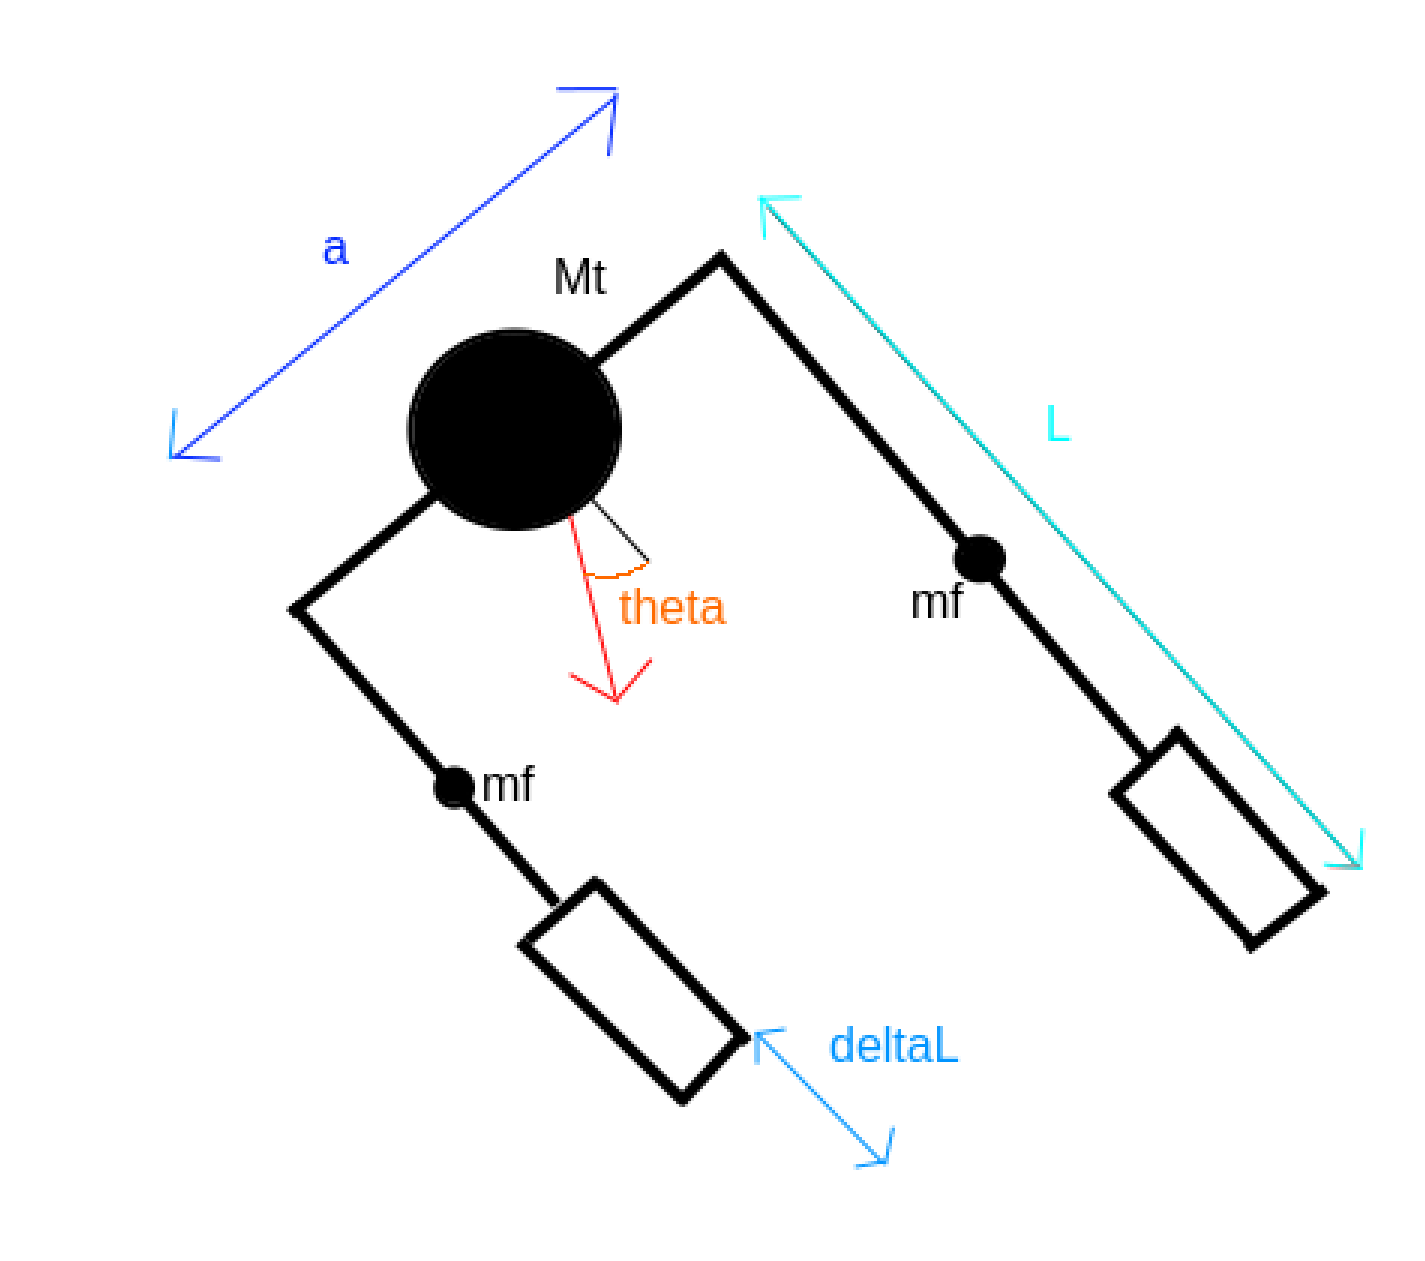
\includegraphics[width=0.55\linewidth]{Figures/ch7_tippingPoint.png}
    \caption{Simplified model of vehicle tipping point}
    \label{fig:vehicleTipping}
\end{figure}
$$
\tan\left( \arctan\left(\frac{\delta L}{a}\right) + \theta \right) > \frac{a \left(M_t + 4m_f\right)}{2 \left( (M_t + 2m_f)L - m_f \delta L \right)}
$$


Parameter Definitions

\begin{itemize}
  \item $a$: Horizontal distance between the legs (along the tipping direction).
  \item $\delta L$: Height difference between the long and short legs.
  \item $L$: Length of the longer legs.
  \item $M_t$: Mass of the vehicle cabin.
  \item $m_f$: Mass of each leg+wheel (assumed identical for all four legs).
  \item $\theta$: Angle between the resulting vector on the CoM and the normal of the plane made by the top of the leg, in the tipping direction. This help to model the gravity if the road is slopped and the centrifugal acceleration:
    \begin{itemize}
      \item $\theta > 0$: tipping is more likely.
      \item $\theta < 0$: tipping is resisted.
    \end{itemize}
\end{itemize}
we can then compute the stability margin on each side with the following.
\begin{align*}
\theta_{\text{critical,left}} &= \arctan\left(\frac{a \left(M_t + 4m_f\right)}{2 \left( (M_t + 2m_f)L - m_f \delta L \right)}\right) - \arctan\left(\frac{\delta L}{a}\right)\\
\theta_{\text{critical,right}} &= \arctan\left(-\frac{a \left(M_t + 4m_f\right)}{2 \left( (M_t + 2m_f)L - m_f \delta L \right)}\right) + \arctan\left(\frac{\delta L}{a}\right) \\
\\
\text{Stability margin on left side} &= \theta_{\text{critical,left}} - \theta \\
\text{Stability margin on right side} &= \theta - \theta_{\text{critical,right}}
\end{align*}
Without surprise, to maximize the stability margin, we should make the vehicle as wide as possible and keep the height of the center of mass as low as possible. But as always it's a matter of tradeoff, the final stability margin will be given by the controller, and thus we can tune these parameters to have just what is necessary to avoid losing the benefit of having a NTV. If the need arose we could make the leg deploy sideway instead of along the body to temporarily increase the width of the vehicle and thus when the system leans the margin also increase. But this is mechanically more complicated as it requires keeping both wheel parallel if we want to avoid adding more non-linear coupling which make the controller more complicated as we wheel also need to compensate for the shift of the contact patch on the wheel.